\documentclass{ntmanuscript}
%\usepackage[acronym,toc]{glossaries}
%\include{acros}
%\makeglossaries
%%%%%%%%%%%%%%%%%%%%%%%%%%%%%%%%%%%
\title{Non-judgemental Dynamic Fuel Cycle Benchmarking}

% Authors. Separated by commas
\author{Anthony Michael Scopatz$^1$}


% Institutes of the authors
\institute{$^1$University of South Carolina, Department of Mechanical 
    Engineering, Nuclear Engineering Program, Columbia, SC 29201}



% Information concerning the person submitting the manuscript
\submitter{Anthony M. Scopatz}
\submitteraddress{541 Main Street, Columbia, SC 29208}
\submitteremail{scopatz@cec.sc.edu}


% No more than three keywords, though each can be a phrase
\keywords{nuclear fuel cycle, gaussian process, dynamic time warping}

\usepackage{color}
\usepackage{graphicx}
\usepackage{booktabs} % nice rules for tables
\usepackage{microtype} % if using PDF
\usepackage{xspace}
\usepackage{listings}
\usepackage{textcomp}
\usepackage{ulem}
\usepackage{amssymb}
\DeclareMathAlphabet{\mathpzc}{OT1}{pzc}{m}{it}

\definecolor{listinggray}{gray}{0.9}
\definecolor{lbcolor}{rgb}{0.9,0.9,0.9}
\lstset{
    %backgroundcolor=\color{lbcolor},
    language={C++},
    tabsize=4,
    rulecolor=\color{black},
    upquote=true,
    aboveskip={1.5\baselineskip},
    belowskip={1.5\baselineskip},
    columns=fixed,
    extendedchars=true,
    breaklines=true,
    prebreak=\raisebox{0ex}[0ex][0ex]{\ensuremath{\hookleftarrow}},
    frame=single,
    showtabs=false,
    showspaces=false,
    showstringspaces=false,
    basicstyle=\scriptsize\ttfamily\color{green!40!black},
    keywordstyle=\color[rgb]{0,0,1.0},
    commentstyle=\color[rgb]{0.133,0.545,0.133},
    stringstyle=\color[rgb]{0.627,0.126,0.941},
    numberstyle=\color[rgb]{0,1,0},
    identifierstyle=\color{black},
    captionpos=t,
}

\newcommand{\code}[1]{\lstinline[basicstyle=\ttfamily\color{green!40!black}]|#1|}
\newcommand{\units}[1] {\:\text{#1}}%
\newcommand{\SN}{S$_N$}
\newcommand{\cyclus}{\textsc{Cyclus}\xspace}
\newcommand{\Cyclus}{\cyclus}
\newcommand{\citeme}{\textcolor{red}{CITE}\xspace}
\newcommand{\cycpp}{\code{cycpp}\xspace}
\newcommand{\TODO}[1] {{\color{red}\textbf{TODO: #1}}}%

\newcommand{\comment}[1]{{\color{green}\textbf{#1}}}

\newcommand{\E}{\mathbb{E}}
\newcommand{\GP}{\mathpzc{GP}}
\newcommand{\LWR}{\mathrm{LWR}}
\newcommand{\FR}{\mathrm{FR}}
\newcommand{\Total}{\mathrm{Total}}
\newcommand{\argmin}{\mathrm{argmin}}
\newcommand{\CYCLUS}{\mathrm{Cyclus}}
\newcommand{\DYMOND}{\mathrm{DYMOND}}
\newcommand{\I}{\mathbf{I}}
\newcommand{\K}{\mathbf{K}}


\date{}
%%%%%%%%%%%%%%%%%%%%%%%%%%%%%%%%%%%
\begin{document}

\begin{abstract}
A method for quickly determining deployment schedules that meet a given 
fuel cycle demand is presented here. This algorithm is fast enough to 
perform \emph{in situ} in low-fidelity fuel cycle simulators. It uses
Gaussian process regression models to predict the prodcution curve as a 
function of time and the number of deployed facilites. The each of these
predictions is measured against the demand curve using the dynamic time
warping distance. The minium distance deployment schedule is evaluated
in a full fuel cycle simulation, whose generated prodcution curve 
then informs the model on the next optimization iteration. The method
converges with five to ten iterations to a total distance less than one 
percent of the total deployable production. A representative once-through
fuel cycle is used to demonstrtate the methodology.
\end{abstract}

\section{Introduction}
\label{intro}

With the recent advent of agent-based nuclear fuel cycle simulators, such as 
Cyclus \cite{DBLP:journals/corr/HuffGCFMOSSW15,cyclus_v1_0}, there comes the 
possibility to make \emph{in situ}, dynamic facility deployment decisions.
This  would more fully model real-world fuel cycles where institutions 
(such as utility companies)
predict future demand and choose their future deployment schedules 
appropriately. However, one of the major challenges to making \emph{in situ}
deployment decisions is the speed at which ``good enough'' decisions can 
be made. This paper proposes three related deployment-specific optimization 
algorithms that can be used for any demand curve and facility type.

The demands of a fuel cycle scenario can often be simply stated, e.g. 
1\% growth in power production [GWe]. Picking a deployment schedule for a 
certain kind of facility (e.g. reactors) can thus be seen as an optimization 
problem of how well the deployment schedule meets the demand. Here, the 
dynamic time warping (DTW) \cite{muller} distance is minimized 
between the demand curve and the regression of a Gaussian Process model (GP) 
\cite{rasmussen2006gaussian} of prior simulations. This minimization produces
a guess for a deployment schedule which is subsequently tested using 
the actual simulator. This process is repeated until an optimal deployment
schedule for the given demand is found.

Importantly, by using the Gaussian process surrogates, the number of 
simulation realizations that must be executed as part of the optimization may 
be reduced to only a handful. Furthermore, it is at least two 
orders-of-magnitude faster to test the model than it is to run a single
low-fidelity fuel cycle simulation. Because of the relative computational 
cheapness, it 
is suitable to be used inside of a fuel cycle simulation. Traditional
\emph{ex situ} optimizers may be able to find more precise solutions but at a
computational cost beyond the scope and need of an \emph{in situ} use case.

Every iteration of the warp optimization of regressed Gaussian processes (WORG) 
method described here has two phases. The first is an estimation phase where 
the Gaussian process model is built and evaluated. The second takes the 
deployment schedule from the estimation phase and runs it in a fuel cycle 
simulator. The results of the simulator of the $s$-th iteration are then 
used to inform the model on the $(s+1)$-th iteration. 

Inside of each estimation phase there are three possible strategies for 
choosing the next deployment schedule.  The first is to sample of the 
space of all possible deployment strategies stochastically and then take the 
best guess.  The second is to search through the inner product of all choices,
picking the best option for each deployment parameter. The third strategy
is to perform the two previous strategies and determine which one has picked
the better guess.

Nuclear fuel cycle demand curve optimization faces many challenges. 
Foremost among these is that even though the demand curve is specified on 
the range of the real numbers, the optimization parameters are fundamentally 
integral in nature. For a discrete time simulator, deployments can only 
be issued in multiples of the size of the time step 
\cite{kelton2000simulation}. Furthermore, 
it is not possible to deploy only part of a facility; the facility is either 
deployed or it is not. While it may be possible to deploy a facility and 
only run it at partial capacity, most fuel cycle models do not support this
for key faciities.  For example, it is unlikely that a utility would build 
a new reactor only to run it at 50\% power. Thus, deployment is an integer 
programming problem, as oppossed to its easier linear programming cousin
\citeme.

Furthermore, the option space is combinatorically large since the 
question is, ``How many facilities should be deployed on each time step?'' 
Even assuming a 50 year deployment schedule where no more than 3 facilities 
are allowed to be deployed each time step, there are more than $10^30$ 
combinations. If every simulation took a very generous 1 sec, simulating 
each option would still take $\approx 3\times10^12$ times the current age
of the universe.

Moreover, because all of the parameters are integral, there is not a 
meaningful formualtion of the Jacobian. Derivitive-free optimizers are 
required. Methods such as particle swarm \citeme, pswarm \citeme, and the 
simplex method all could work.  However, typical implementations require
more evaluations of the objective function (i.e. fuel cycle simulations)
than are within an \emph{in situ} budget. 

Even the usual case of 
Gaussian process optimization (sometimes known as kriging) will still 
require too many full realizations in order to form an accurate model.
WORG, on the other hand, using the dynamic time warping distance as a 
more separative measure of how two time series differ than just a simple
L1 norm (or similar). This drives the estimation phase to make better choices
sooner, and help converge to a reasonable deployment schedule sooner. 
The stochastic strategy for WORG also utilizes Gaussian processes to 
weight the choice of parameters.  This guides the guesses for the deployment
schedules such that fewer guesses are needed, while not fully restricting 
any option.  So while WORG relies on Gaussian processes, it does so in a way
that is distinct from normal kriging. WORG
takes advantage of the \emph{a priori} knowledge that a deployment 
schedule is requested to meet a demand curve. 

The structure of the WORG method is detailed in \S\ref{method}. 
The different strategies for selecting a best-guess estimate of the 
deployment schedule are then discussed in \S\ref{selecting}. Performance
and results of the method for a sample once-through fuel cycle scenario 
are presented in \S\ref{results}. Finally, \S\ref{conclusion} summarizes
WORG and list opportunities for future work.

%\subsection{Gaussian Process Regression}
\label{gp}

Evaluating the production curve for a specific kind of facility using 
full fuel cycle simulations is relatively expensive, even in the 
computationally cheapest case of low-fidelity simulations. This is because a 
fuel cycle realization 
typically computes many features that, though coupled to the production 
curve, are not directly the production curve. For example, the mass balance of 
the fuel cycle physically bounds the electricity production. However, the    
mass balances are not explicitly taken into account when trying to meet
a demand curve.

Alternatively, surrogate models that predict the production curve directly
have many orders-of-magnitude fewer operations by virtue of not computing
implicit physical characteristics. This is not to say that the surrogate 
models are correct.  Rather, they are simply good enough to drive a demand
curve 
optimization. Surrogate models are used here inform a simulator about where
in the parameter space to look next. Truth about production curves should
still be derived from the fuel cycle simulator and not the surrogate model.
In the WORG algorithm, Gaussian processes are used to form the model. 

Gaussian processes are more fully covered elsewhere 
\cite{rasmussen2006gaussian}. Using Gaussian process for optimization has 
also been previously explored \cite{osborne2009gaussian}, though such studies 
tend not to 
investigate the intergal problems posed by facility deployment. As with 
dynamic time warping, a minimal but sufficient introduction to GP is presented 
for the purposes of the deployment optimization.
Conside the case of $Z$ simulations indexed by $z$ that each have a 
$\Theta_z$ deployment schedule and $g_z(t, \Theta_z)$ production curve.

A Gaussian process of these $Z$ simulations is set by its mean and 
covariance functions. The mean function is denoted as $\mu(t, \Theta)$ and 
is the expectation value $\E$ of 
the series of $G$ inputs:
\begin{equation}
\label{G}
G = \left\{g_1(t, \Theta_1), g_2(t, \Theta_2), \ldots, 
           g_Z(t, \Theta_Z)\right\}
\end{equation}
The covariance function is denoted $k(t, \Theta, t^\prime, \Theta^\prime)$ 
and is the expected value of the input to the mean. The mean and 
covariance can be expressed as
in Equations \ref{mean-func} \& \ref{covar-func} respectively.
\begin{equation}
\label{mean-func}
\mu(t, \Theta) = \E G
\end{equation}
\begin{equation}
\label{covar-func}
k(t, \Theta, t^\prime, \Theta^\prime) = 
    \E\left[(g_z(t, \Theta) - \mu(t, \Theta))
            (g_z(t^\prime, \Theta^\prime) - \mu(t^\prime, \Theta^\prime))
      \right]
\end{equation}
Note that in the above, the Gaussian process is itself $P+1$ dimensional, 
since the means and covariance are a function of both the deployment 
schedule ($P$) and time ($+1$).

The Gaussian process $\GP$ approximates the production curve 
given $Z$ simulators. Allow $*$ to indicate that the a quantity comes from 
the model as opposed to coming from the simulator information. A model 
production curve can then be written using either functional or operator
notation, as appropriate:
\begin{equation}
\label{gp-def-approx}
g_*(t, \Theta) \approx \GP\left(\mu(t, \Theta), 
                                 k(t, \Theta, t^\prime, \Theta^\prime)\right) 
                \equiv \GP G
\end{equation}
In machine learning terminology, $G$ serves as the training set for the 
GP model.

Now, when performing a regression on Gaussian processes, 
the nominal functional form for the covariance must be given. 
Such a functional form is also known as the the kernel function.
The kernel contains the \emph{hyperparameters} that are solved for to 
obtained a best-fit Gaussian process. The hyperparameters themselves are
defined based on the definition of the kernel function. Hyperparameter 
values are found via a regression of the maximal likelihood of 
the production curve. Any functional form could potentially serve as a kernel
function. However, a generally useful form is the is the exponential 
squared. This kernel can be seen in Equation \ref{exp2-kernel} with 
hyperparameters $\ell$ and $\sigma^2$ for a vector of parameters $r$:
\begin{equation}
\label{exp2-kernel}
k(r, r^\prime) = \sigma^2 \exp\left[-\frac{1}{2\ell}(r - r^\prime)^2 \right]
\end{equation}
However, other kernels such as the Mat\'ern $3/2$ kernel and Mat\'ern $5/2$
kernel \cite{paciorek2004nonstationary} were observed to be more robust for 
the WORG method. These can be seen in Equations \ref{matern-32} and 
\ref{matern-52} respectively.
\begin{equation}
\label{matern-32}
k(r, r^\prime) = \sigma^2 
                 \left(1 + \frac{\sqrt{3}}{\ell}|r - r^\prime|\right)
                 \exp\left(-\frac{\sqrt{3}}{\ell}|r - r^\prime|\right)
\end{equation}
\begin{equation}
\label{matern-52}
k(r, r^\prime) = \sigma^2 
                 \left(1 + \frac{\sqrt{5}}{\ell}|r - r^\prime|
                         + \frac{5}{3\ell^2}|r - r^\prime|^2\right)
                 \exp\left(-\frac{\sqrt{5}}{\ell}|r - r^\prime|\right)
\end{equation}

From here, say that $\K$ is a covariance matrix 
such that the element at the $r$-th row and $r^\prime$-th column is 
given by whichever kernel is chosen from 
Equations \ref{exp2-kernel}-\ref{matern-52}. Then the 
log likelihood $\log q$ of the obtaining the training set production curves 
$G$ for a given time grid $\mathbf{t}$ and deployment schedule is as 
seen in Equation \ref{log-q}.
\begin{equation}
\label{log-q}
\log q(G|\mathbf{t}, \Theta) 
    = -\frac{1}{2}G^\top\left(\K + \tau^2\I\right)^{-1}G
      -\frac{1}{2}\log\left|\K + \tau^2\I\right|
      -\frac{ZTP}{2}\log 2\pi
\end{equation}
Here, $\tau$ is the uncertainty in the production curves coming from the 
simulations themselves. As most simulators do not report such uncertainties, 
$\tau$ may be set to floating point precision. $\I$ is the usual identity 
matrix. The hyperparameters $\ell$ and $\sigma^2$ are then adjusted via 
standard real-valued optimization methods such that Equation \ref{log-q} is 
minimized. 
This regression of the Gaussian process itself yields the most likely 
model of the production curve, knowing only a limited number simulations.

However, the purpose of such a Gaussian process regression is to evaluate 
the production curve at points in time and for deployment schedules that 
have not been simulated. Take a time grid $\mathbf{t_*}$ and a hypothetical
deployment schedule $\Theta_*$. Now call the covariance vector between
the training set and the model evaluation    
$\mathbf{k}_* = \mathbf{k}(\mathbf{t_*}, \Theta_*)$. 
The production curve predicted by this Gaussian process is then given by
the following:
\begin{equation}
\label{metric-model}
\mathbf{g}_*(\mathbf{t}_*, \Theta_*) = 
    \mathbf{k}_*^\top \left(\K + \tau^2\I\right)^{-1}G
\end{equation}
Equations \ref{mean-func}-\ref{metric-model} are derived and discussed fully
in \cite{rasmussen2006gaussian}. 

However, implementing the above Gaussian process mathematics for the specific
case of the WORG algorithm 
is not needed.  Off-the-shelf Gaussian process modeling software 
libraries already exist and are applicable to the regression problem here.
Scikit-learn v0.17 \cite{scikit-learn} and George v0.2.1 \cite{hodlr} 
implement such a method and have a Python interface. George is specialized 
around Gaussian processes, and thus is preferred for WORG over scikit-learn, 
which is a general purpose machine learning library.

As an example, consider a Gaussian process between two power production 
curves similar to the example used in \S\ref{dtw}. The first is a nominal 1\% growth 
in GWe for 50 years starting at 
90 GWe in 2016. The second curve under produces the first curve by 10\% 
for the first 25 years and over produces by 10\% for the last 25 years.
Additionally, assume that there is a 10\% error on the training data set.
This will produce a model of the mean and covariance that splits the 
difference between these two curves. This example may be seen graphically
in Figure \ref{gwe-model-}.

\begin{figure}[htb]
\centering
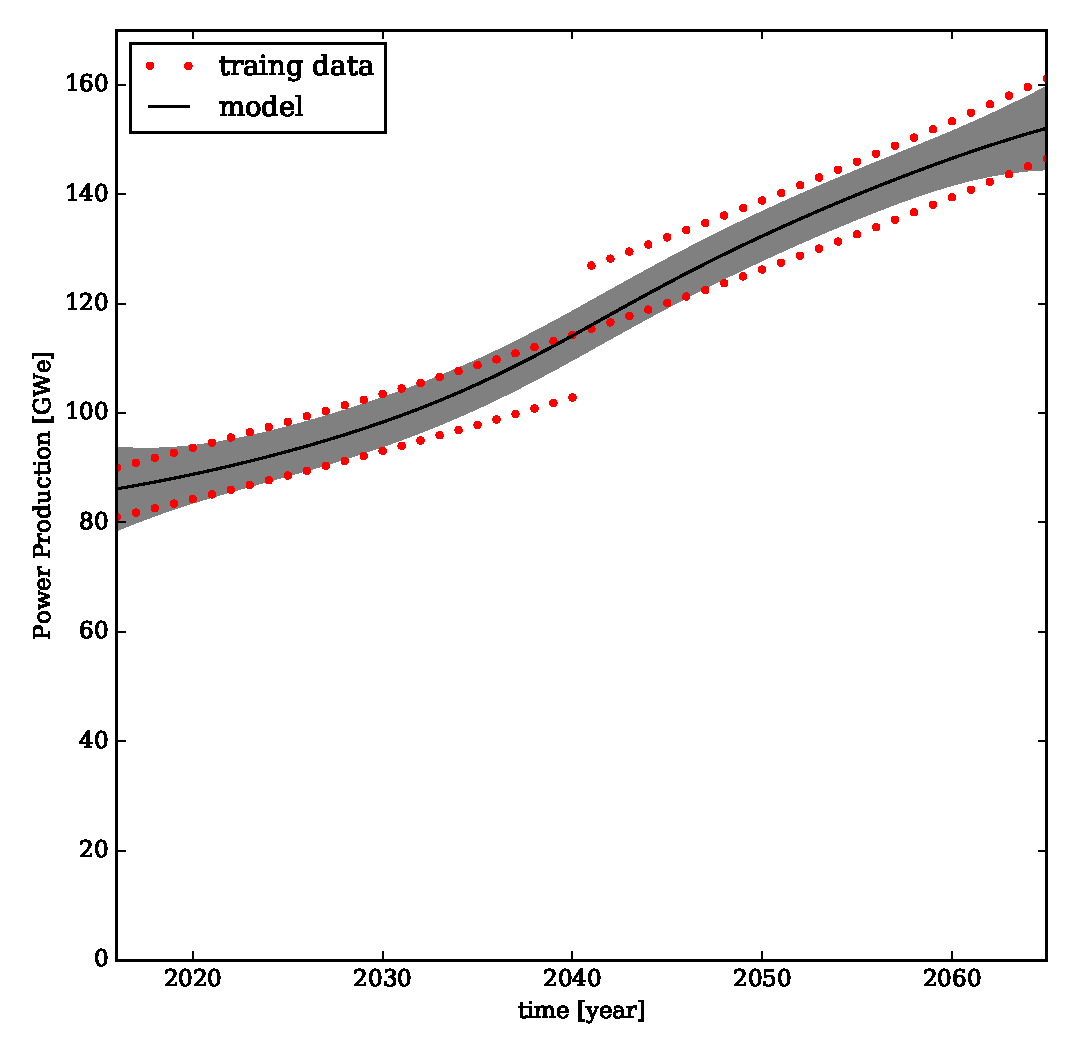
\includegraphics[width=0.9\textwidth]{gwe-model-.eps}
\caption{The Gaussian process model of a 1\% growth curve along with the
an initial 10\% under production followed by a 10\% under production. 
The model is represented by the black line that runs between the red 
training points. Two standard deviations form the model are displayed as the
gray region.}
\label{gwe-model-}
\end{figure}

The simple example above does not take advantage of an important 
feature of Gaussian processes. Namely, it is not limited to two production
curves in the training set.  As many as desirable may be used.  This will
allow the WORG algorithm to dynamically adjust the number of $Z$ simulations 
which are used to predict the next deployment schedule. WORG is thus capabale
of 
effortlessly expanding $Z$ when new and useful simulations yield valuable production
curves.  However, it also enables $Z$ to contract to discard production
curves that would drive the deployment schedule away from an optimum.

Now that the Gaussian process regression and dynamic time warping tools have 
been added to the toolbox, the architecture of the WORG algorithm can 
itself be described.

\clearpage

%\subsection{Dynamic Time Warping}
\label{dtw}

The question of how to take the difference between the demand curve and
the production curve is an important one. The na\"ive option is to simply
take the $L_1$ norm of the difference between these two time series, as
seen in Equation \ref{delta-l1}.  However, since the $g(t, \Theta)$ computed
from a simulation is expensive, any operation that can meaningfully
exacerbate the difference between time series helps drive down the number
of optimization iterations.

Dynamic time warping is just such a mechanism. It computes
a distance between any two time series which compounds the separation
between the two. Additionally, the time series are not required to be of the
same length, though for optimization purposes there is no reason for them
not to be. DTW gives a measure of the amount that one time series would need to
be warped to become the other time series. It is, therefore, a holistic
measure that operates over all times. Dynamic time warping
is more fully covered in \cite{muller}.  However, an
optimization-relevant introduction is given here.

For the time series $f$ and $g$, there are three parts to dynamic time
warping. The first is the distance $d$, which will be minimized. The second
is a cost matrix $C$ that helps compute $d$ by indicating how far a point
on $f$ is from another point on $g$. Thirdly, the warp path $u$ is the
minimal cost curve through the $C$ matrix from the fist point in time to
the last. The DTW distance can thus be interpreted as the
total cost of traveling the warp path.

The first step in computing a dynamic time warp distance is to
assemble the cost matrix. Say that the demand time series $f$ has
length $A$ indexed by $a$, and the production time series $g$ has
length $B$ indexed by $b$. For the optimization problem here, $A$ and $B$
are in practice both equal to $T$.  However, it is useful to have $a$ and
$b$ index the two time series separately. Now denote an $A\times B$ matrix
$\Delta L$ as the $L_1$ norm of the difference between $f$ and $g$:
\begin{equation}
\label{delta-l1}
\Delta L_{a,b} = \left|f(a) - g(b, \Theta)\right|_1
\end{equation}
Since $\Delta L$ uses the $L_1$ norm, $f$ and $g$ may return vector
data. This enables multi-objective optimization. However it is recommended
that the components of the $f$ and $g$ are weighted, normalized, or otherwise
directly comparable.

The cost matrix $C$ may now be defined as the $A\times B$ sized matrix
which follows the recursion relations seen in Equation \ref{cost-matrix}.
\begin{equation}
\label{cost-matrix}
\begin{split}
C_{1,1} & = \Delta L_{1,1}\\
C_{1,b+1} & = \Delta L_{1,b} + C_{1,b}\\
C_{a+1,1} & = \Delta L_{a,1} + C_{a,1}\\
C_{a+1,b+1} & = \Delta L_{a,b} + \min\left[C_{a,b}, C_{a+1,b}, C_{a,b+1}\right]
\end{split}
\end{equation}
The boundary conditions above are the same as setting an infinite cost to
any $a \le 0$ or $b \le 0$. The cost matrix $C$ has the same units as the
demand curve. However, the scale of $C$ is
larger than the demand,
except for in the fiducial case. This is because the cost matrix compounds the
minimum value of previous entries.

Knowing a cost matrix, the warp path can be computed by traversing the
matrix backwards from the $(A, B)$ corner to the $(1, 1)$ corner.
If the length of the warp is $I$ indexed by $i$, the warp path itself
can be thought of as a sequence of coordinate points $u_i$. For a given
point $u_i$ in the warp path, the previous point $u_{i-1}$ may be found by
picking the minimum cost point among the locations one column over $(a,b-1)$,
one row over $(a-1,b)$, and one previous diagonal element to $(a-1,b-1)$.
Equation \ref{warp-path} expresses this mathematically.
\begin{equation}
\label{warp-path}
u_{i-1} = \argmin\left[C_{a-1,b-1}, C_{a-1,b}, C_{a,b-1}\right]
\end{equation}
The maximum possible length of $u$ is thus $\max(I) = A + B$.
The minimum possible length, though, is $\min(I) = \sqrt{A^2 + B^2}$.

The dynamic time warping distance distance $d$ can now be stated as the
cost of the final entry of the warp path normalized by the maximum possible
length of the warp path.
\begin{equation}
\label{d-calc-ab}
d(f, g) = \frac{C_{A,B}}{A + B}
\end{equation}
However, because the demand curve and the production curve
are often defined on the same time grid, $d$ can be further
reduced to the following:
\begin{equation}
\label{d-calc}
d(f, g) = \frac{C_{T,T}}{2T}
\end{equation}
Therefore, $d$ has the same units as the demand curve, production curve,
and cost matrix.

As an example, take a 1\% growth that starts with 90 GWe in the year
2016 as the demand curve. Then consider a production curve that
under-produces the demand by 5\% for 25 years before switching to
over-producing this curve by 5\% for the next 25 years.
Figure \ref{cost-demand-to-production} shows the dynamic time warping
cost matrix between these two time series as a heat map.

\begin{figure}[htb]
\centering
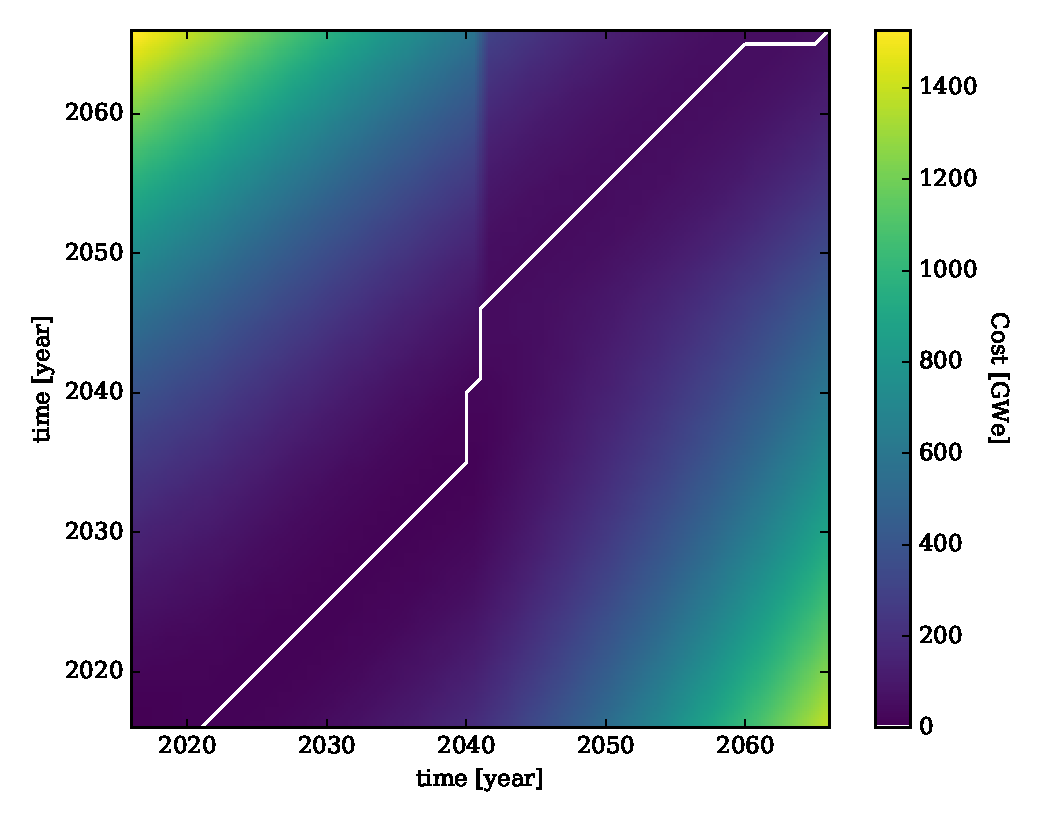
\includegraphics[width=0.9\textwidth]{cost-demand-to-production.eps}
\caption{Heat map of the cost matrix between a 1\% growth demand curve and
a production curve the under produces by 5\% for the first 25 years and then
over produces for the second 25 years.
The warp path $u$ is superimposed as the white curve on top of the
cost matrix.}
\label{cost-demand-to-production}
\end{figure}

Additionally, the warp path between the example demand and production
curves is presented as the white curve on top of the heat map in
Figure \ref{cost-demand-to-production}.
Recognize that $u$ is monotonic along both time axes. Furthermore, the precise
path of $u$ minimizes the cost matrix at every step. Regions of increased
cost in the cost matrix can be seen to repel the warp path. The
distance $d$ between the demand and production curves here happens
to be 0.756 GWe.

Dynamic time warping distance can therefore be used as an objective function
to minimize for any demand and production curves. However, using full
simulations to find $g(t, \Theta)$ remains expensive, even though DTW itself
is computationally cheap. Therefore, a mechanism to reduce the overhead
from production curve evaluation is needed.

\section{Conclusions \& Future Work}
\label{conclusion}

The WORG method provides a deployment schedule optimizer that converges
both closely enough and fast enough to be used inside
of a nuclear fuel cycle simulator. The algorithm can consistently obtain
tolerances of half-a-percent to a percent (1 GWe distances for over 200 GWe
deployable) for the once-through fuel cycle featured here within only five to
ten simulations. Such optimization problems are made
more challenging due to the integral nature of facility deployment and
that any demand curve may be requested.

WORG works by setting up a Gaussian process to model the production
as a function of time and the deployment schedule. This model may then
be evaluated orders of magnitude faster than running a full simulation, enabling
the search over many potential deployment schedules. The quality of these
possible schedules is evaluated based on the dynamic time warping distance
to the demand curve. The lowest distance curve is then evaluated in a
full fuel cycle simulation. The production curve that is computed by the
simulator in turn goes on to update the Gaussian process model and the
cycle repeats until the limiting conditions are met.

However, choosing the deployment schedules to estimate with the Gaussian
process may be performed in a number of ways. A blind approach would
simply be to choose such schedules randomly from a univariate. However,
the WORG method has more information available to it that helps drive
down the number of loop iterations. The first method discussed remains
stochastic but uses the inverse DTW distances of the GP model to
weight the deployment options, falling back to a Poisson distribution as
necessary. This second method minimizes the model distance for each point
in time from start to end, iteratively building up a solution. Finally,
another estimation strategy tries both previous options and chooses the
best result, forcing the stochastic method two of every four iterations
to avoid deterministic loops.  It is this last all-of-the-above method
that is seen to converge the fastest and to the lowest distance in most
cases.

It is important to note that the WORG algorithm is applicable to any
demand curves and fuel cycle facility types. It is not restricted to
reactors and power. Enrichment and separative work units, reprocessing
and separations capacity, and deep geologic repositories and their
space could be deployed via the WORG method for any applicable demand
curve. Furthermore, several of these demands and deployments can be
examined simultaneously. For instance, deployment schedules for light-water,
fast reactors, pebble-bed reactors, and separations facilities may be optimized
together on the joint
bases of minimizing cost, minimizing separated transuranics, and achieiving
a specified power demand. The WORG algorithm fuilly supports such mutlivariate
problems. Reactors and power generation were chosen for study here as the
representative keystone example, though the algorithm is not tied to this
particular problem.

The speed of convergence of the WORG algorithm is effectively required for
high-fidelity simulation optimization. Single realizations may take hours or
longer to run. Executing hundred, thousands, or more realizations becomes
impractical. On the other hand, lower fidelity simulations that have short
execution times may be perfectly well optimizied by an \emph{ex situ}
method. With fast run times, WORG would be implemented \emph{in situ} as
a mechanism for automation and avoiding external wrapper codes implicit
in an \emph{ex situ} optimizer. The speed of convergence for lower fidelity
simulations, while desirable conceptually, is not required in practice.

The next major step for this work is to actually employ the WORG method in
a fuel cycle simulator.  However, to the best knowledge of the
author, no existing simulator is capable of spawning forks of itself
during run time, rejoining the processes, and evaluating the results of the
child simulations in the parent simulation. Concisely, while many simulators
are `dynamic' in the fuel cycle sense, none are `dynamic' in the programming
language sense. This latter usage of the term is what is required to
take advantage of any sophisticated \emph{in situ} deployment optimizer.
The Cyclus fuel cycle simulator looks most promising as a platform
for such work to be undertaken. However, many technical roadblocks
on the software side remain, even for Cyclus.

Additionally, the WORG method does not utilize an expected decomissioning
schedule. If it is known prior to the simulation, this information
could help focus on a deployment schedule solution faster and more precisely.
Futrue work on WORG will consider optionally providing the decomisiong inforation.
This will likely affect the initial two optimizer cases and the
$M_p$ and $N_p$ deployment bounds.

Furthermore, adding \emph{in situ} capability also adds the additional
degree of freedom of how often to run the deployment schedule optimizer.
Running WORG each and every
time step seems excessive \emph{a priori}. Is every year, five years,
or ten years sufficient? How does this degree of freedom balance with the
time horizon $T$ specified in the optimizer? These questions remain unanswered, even
in a heuristic sense, and thus the frequency of optimization will be a key
parameter in a future \emph{in situ} study.

%% Uncomment the following to use.
\section*{Acknowledgements}
\label{acknow}


%%%%%%%%%%%%%%%%%%%%%%%%%%%%%%%%%%%%%%%%%%%%%%%%%%%%%%%%%%%%%%%%%%%%%%%%%%%%%%%%
\bibliographystyle{ans}
\bibliography{refs}
\end{document}
